\documentclass[varwidth]{standalone}

\usepackage{tikz}
\usepackage{tikz-feynhand}
\usepackage{physics}

\begin{document}
\centering
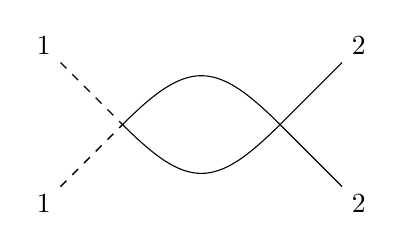
\begin{tikzpicture}
  \begin{feynhand}
    % vertices
    \vertex (p11) at (-1,1) {1};
    \vertex (p12) at (-1,-1) {1};
    \vertex (p21) at (3,1) {2};
    \vertex (p22) at (3,-1) {2};
    \vertex (a) at (0,0);
    \vertex (b) at (2,0);
    % particles
    \propag [sca] (p11) to (a);
    \propag [sca] (p12) to (a);
    \propag (b) to (p21);
    \propag (b) to (p22);
    % loop
    \propag (a) to [in=135, out=045, looseness=1.5] (b);
    \propag (b) to [out=225, in=315, looseness=1.5] (a);
  \end{feynhand}
\end{tikzpicture}
\begin{tikzpicture}
  \begin{feynhand}
    % vertices
    \vertex (p11) at (-1,1) {1};
    \vertex (p12) at (-1,-1) {1};
    \vertex (p21) at (3,1) {2};
    \vertex (p22) at (3,-1) {2};
    \vertex (a) at (0,0);
    \vertex (b) at (2,0);
    % particles
    \propag [sca] (p11) to (a);
    \propag [sca] (p12) to (a);
    \propag (b) to (p21);
    \propag (b) to (p22);
    % loop
    \propag [sca] (a) to [in=135, out=045, looseness=1.5] (b);
    \propag [sca] (b) to [out=225, in=315, looseness=1.5] (a);
  \end{feynhand}
\end{tikzpicture}
\\
\begin{tikzpicture}
  \begin{feynhand}
    % vertices
    \vertex (p11) at (1.5,0) {2}; \vertex (p21) at (1.5,1.5) {2};
    \vertex (p12) at (-1.5,0) {1}; \vertex (p22) at (-1.5,1.5) {1};
    \vertex (a) at (0,0); \vertex (b) at (0,1.5);
    % particles
    \propag (p11) to (a);
    \propag [sca] (p12) to (a);
    \propag (b) to (p21);
    \propag [sca] (b) to (p22);
    % loop
    \propag [sca] (a) to [in=315, out=45, looseness=1] (b);
    \propag (b) to [out=225, in=125, looseness=1] (a);
  \end{feynhand}
\end{tikzpicture}
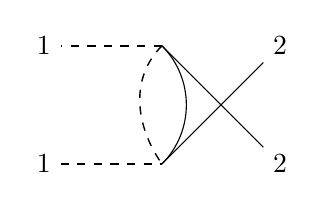
\begin{tikzpicture}
  \begin{feynhand}
    % vertices
    \vertex (p11) at (1.5,0) {2}; \vertex (p21) at (1.5,1.5) {2};
    \vertex (p12) at (-1.5,0) {1}; \vertex (p22) at (-1.5,1.5) {1};
    \vertex (a) at (0,0); \vertex (b) at (0,1.5);
    % particles
    \propag (p21) to (a);
    \propag [sca] (p12) to (a);
    \propag (b) to (p11);
    \propag [sca] (b) to (p22);
    % loop
    \propag (a) to [in=315, out=45, looseness=1] (b);
    \propag [sca] (b) to [out=225, in=125, looseness=1] (a);
  \end{feynhand}
\end{tikzpicture}
\end{document}
